\documentclass[a4paper, oneside, final]{scrartcl}
\usepackage{scrpage2}
\usepackage{geometry}                % See geometry.pdf to learn the layout options. There are lots.
\geometry{a4paper}
\usepackage{graphicx}
\usepackage{amssymb}
\usepackage{epstopdf}
\usepackage{xcolor}
\usepackage{hyperref}
\usepackage{palatino}
\usepackage{titlesec}
\geometry{a4paper,top=2cm,bottom=3.4cm}

\DeclareGraphicsRule{.tif}{png}{.png}{`convert #1 `dirname #1`/`basename #1 .tif`.png}

\hypersetup{
   pdfpagemode=UseOutlines,
   pdfpagelayout=TwoPageRight,
   pdfstartview=Fit,
   plainpages=false,       
   colorlinks
}

\usepackage{colortbl}
\usepackage{color}
\definecolor{dunkelblau}{rgb}{0.1,0.80,0.75}
\definecolor{bordeaux}{rgb}{0.50,0.10,0.10}
\definecolor{gruen}{rgb}{0.20,0.50,0.20}
\definecolor{dunkelgrau}{rgb}{0.35,0.35,0.35}
\definecolor{hellgrau}{rgb}{0.45,0.45,0.45}
\hypersetup{
  linkcolor=black,
  filecolor=black,
  urlcolor=dunkelblau,
  citecolor=black,
}
\pagestyle{scrheadings}
% ------------------

\begin{document}

\title{Getting started with SixTrack}
\author{\large{compiled by R.~Kwee}}

\date{\large{\today}}
        \maketitle


\setlength{\parindent}{0cm}
{\LARGE{\textbf{Preamble}}}\\

\noindent This document is for Sixtrack beginners. See also Roderik's list of ``essential references''.
\section{Optics file}

An input to SixTrack is a file that contains the optics configuration, generated by MadX. Use the \texttt{sixtrack} command within MadX, see also this {\href{http://frs.home.cern.ch/frs/Xdoc/c6t/c6t.html}{description}}. The file \texttt{fc.2} must be renamed for SixTrack to \texttt{fort.2}.

\section{SixTrack}

\subsection{SixTrack Source Code SVN}

The source code of SixTrack can be downloaded from\\ {\href{https://svn.cern.ch/reps/SixTrack/trunk/SixTrack}{\texttt{https://svn.cern.ch/reps/SixTrack/trunk/SixTrack}}. \newline

To compile, run:\\
\texttt{./make\_six gfortran collimat}\newline

During the compilation, the actual fortran files are extracted from the \texttt{sixtrack.s} file into a subdirectory SixTrack\_XXXX depending on the compilation flags. The easiest way to access the code is to look at the extracted file \texttt{track.f} in the subdirectory. 

\subsection{Run SixTrack}
The SixTrack binary executable needs three input files without explicitly handing them over as arguments:

\begin{itemize}
\item \texttt{fort.2}: MadX output file with optics configuration.
\item \texttt{fort.3}: SixTrack configuration file including beam definition (energy, size, distribution), number of packs (1 pack corresponds to 64 particles) , number of turns and the \textit{collimation block}. The parameters of the collimation block are decribed at the LHC collimation {\href{http://lhc-collimation-project.web.cern.ch/lhc-collimation-project/code-tracking-2012.php}{webpage}}.
\item \texttt{CollDB\_V6.503\_lowb\_st.b1.data}: This file name must be defined in the source code of SixTrack. The file contains the collimators names and properties.
\end{itemize}

To launch the executable and save the output one can e.g.~execute: \\
\texttt{./SixTrack\_4411\_coll\_gfortran\_O4 >| screenout} \\

This will produce the following output files:

\begin{enumerate}
\item \texttt{all\_absorptions.dat}
\item \texttt{all\_impacts.dat}
\item \texttt{amplitude2.dat}
\item \texttt{amplitude.dat}
\item \texttt{beta\_beat.dat}

\item \texttt{betafunctions.dat} Contains $\beta_x$ and $\beta_y$ along $s$ at each beamline element (possibly centre). The header looks like \texttt{\# 1=ielem 2=name 3=s 4=TBETAX 5=TBETAY}.

\item \texttt{betatron.dat}
\item \texttt{collgaps.dat} Associates collimator geometry information with main optics parameters. First colum has the collimator ID (according to the appearance in the collimator DB file). It associates to $\beta_x$, $\beta_y$, halfgap, material, length, beam size $\sigma_x$ and $\sigma_y$ (?), tilts and nsig (?). The $\beta$-values are a subset of \texttt{betafunctions.dat}.

\item \texttt{collimator-temp.db}
\item \texttt{collsettings.dat}
\item \texttt{colltrack.out}

\item \texttt{coll\_summary.dat} This file contains the following information: \texttt{1=icoll} is the ID of the collimator, \texttt{2=collname}, collimation name, \texttt{3=nimp}, number of impacting particles, \texttt{4=nabs}, number of absorbed particles, \texttt{5=imp\_av} average impact parameter, \texttt{6=imp\_sig} average impact parameter in $\sigma$, \texttt{7=length}, length of collimator.

\item \texttt{dist0.dat} Contains phase-space information of the initial halo distribution. The colums correspond to \texttt{X[m]   Xp[rad]   Y [m]   Yp[rad]   s in bucket [m]  E[MeV]}.

\item \texttt{distn.dat}
\item \texttt{efficiency.dat} 

\item \texttt{FLUKA\_impacts.dat} This file contains information of lost particles for energy deposition studies. 

\item \texttt{FirstImpacts\_AcceleratorFrame.dat}
\item \texttt{FirstImpacts.dat} This file will (if set so in the source code of SixTrack) a line for each halo particle that impact for the first time on an collimator. Some of them are able to leave the collimators, some of them are absorbed. Thus, the number of lines indicates the total number of halo particles that should be cleaned.

\item \texttt{impact.dat}
\item \texttt{orbitchecking.dat}
\item \texttt{pencilbeam\_distr.dat}
\item \texttt{sigmasettings.out}
\item \texttt{survival.dat} In two colums of this file, it is counted down how many halo particles actually continue tracking even though they have hit a collimator or are lost somewhere else. It indicates how many particles are left after a certain number of turns.

\item \texttt{tracks2.dat} This is usually a massive file with information of all halo particles per turn. There are \texttt{\# 1=name 2=turn 3=s 4=x 5=xp 6=y 7=yp 8=DE/E 9=type} with no.~1 being the particle ID.
\item \texttt{twisslike.out}
\end{enumerate}


\begin{figure}
\begin{center}
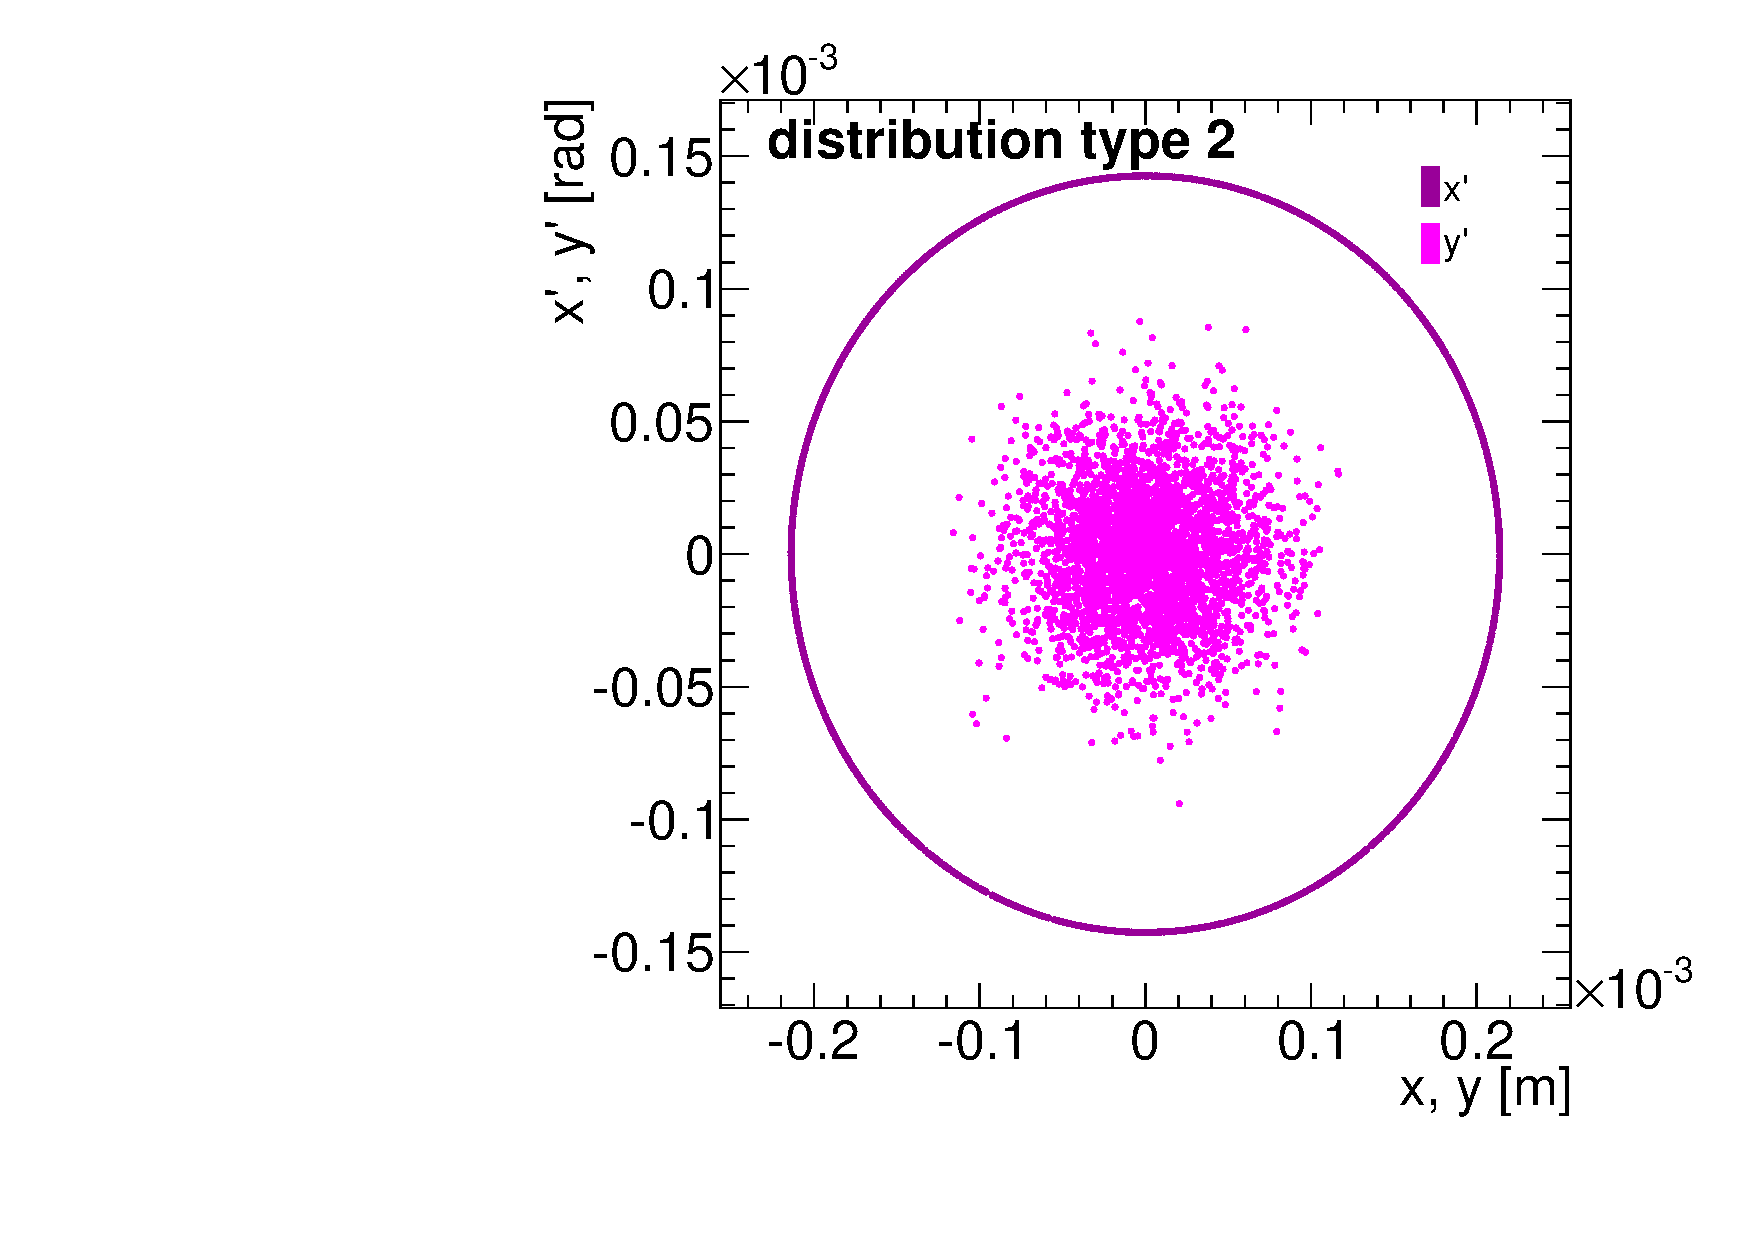
\includegraphics[width=0.48\textwidth]{figures/phasespace_d2}
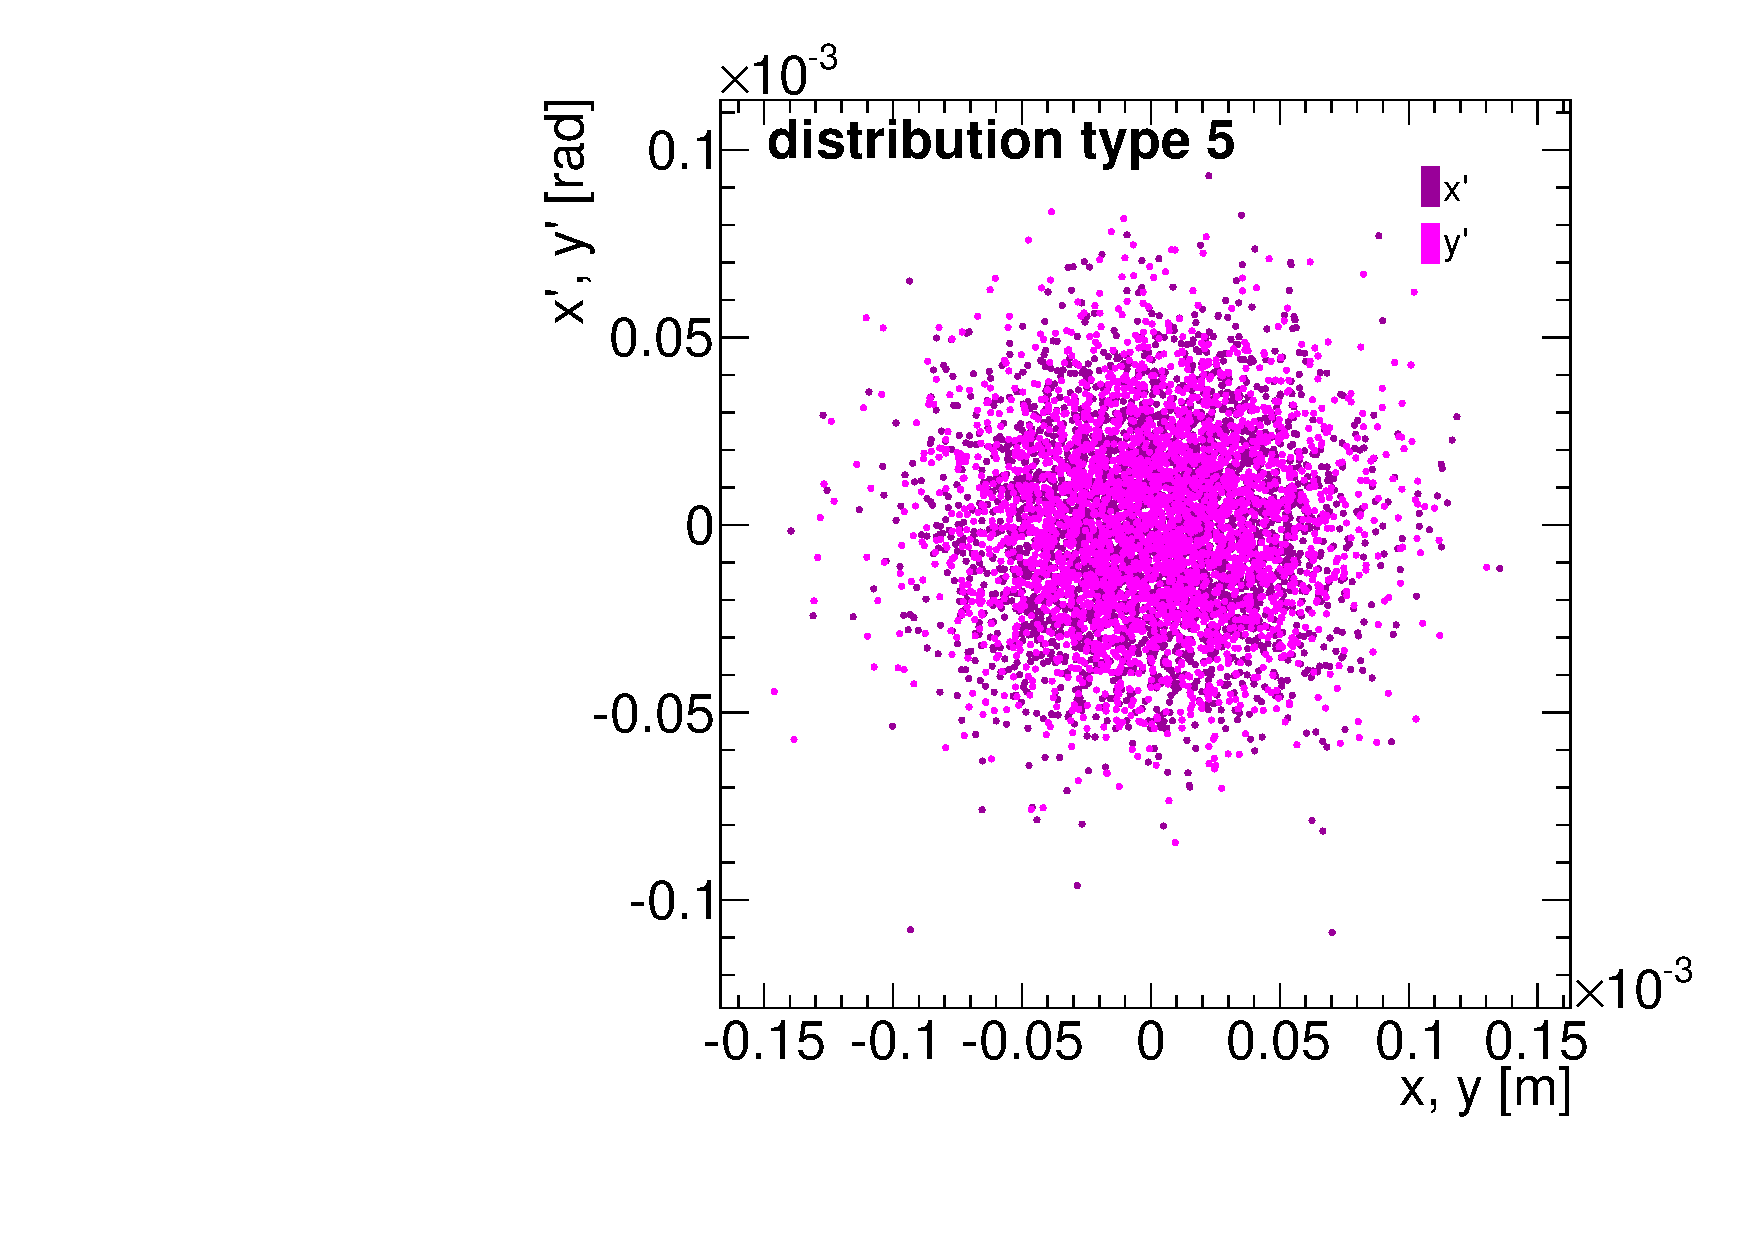
\includegraphics[width=0.48\textwidth]{figures/phasespace_d5}
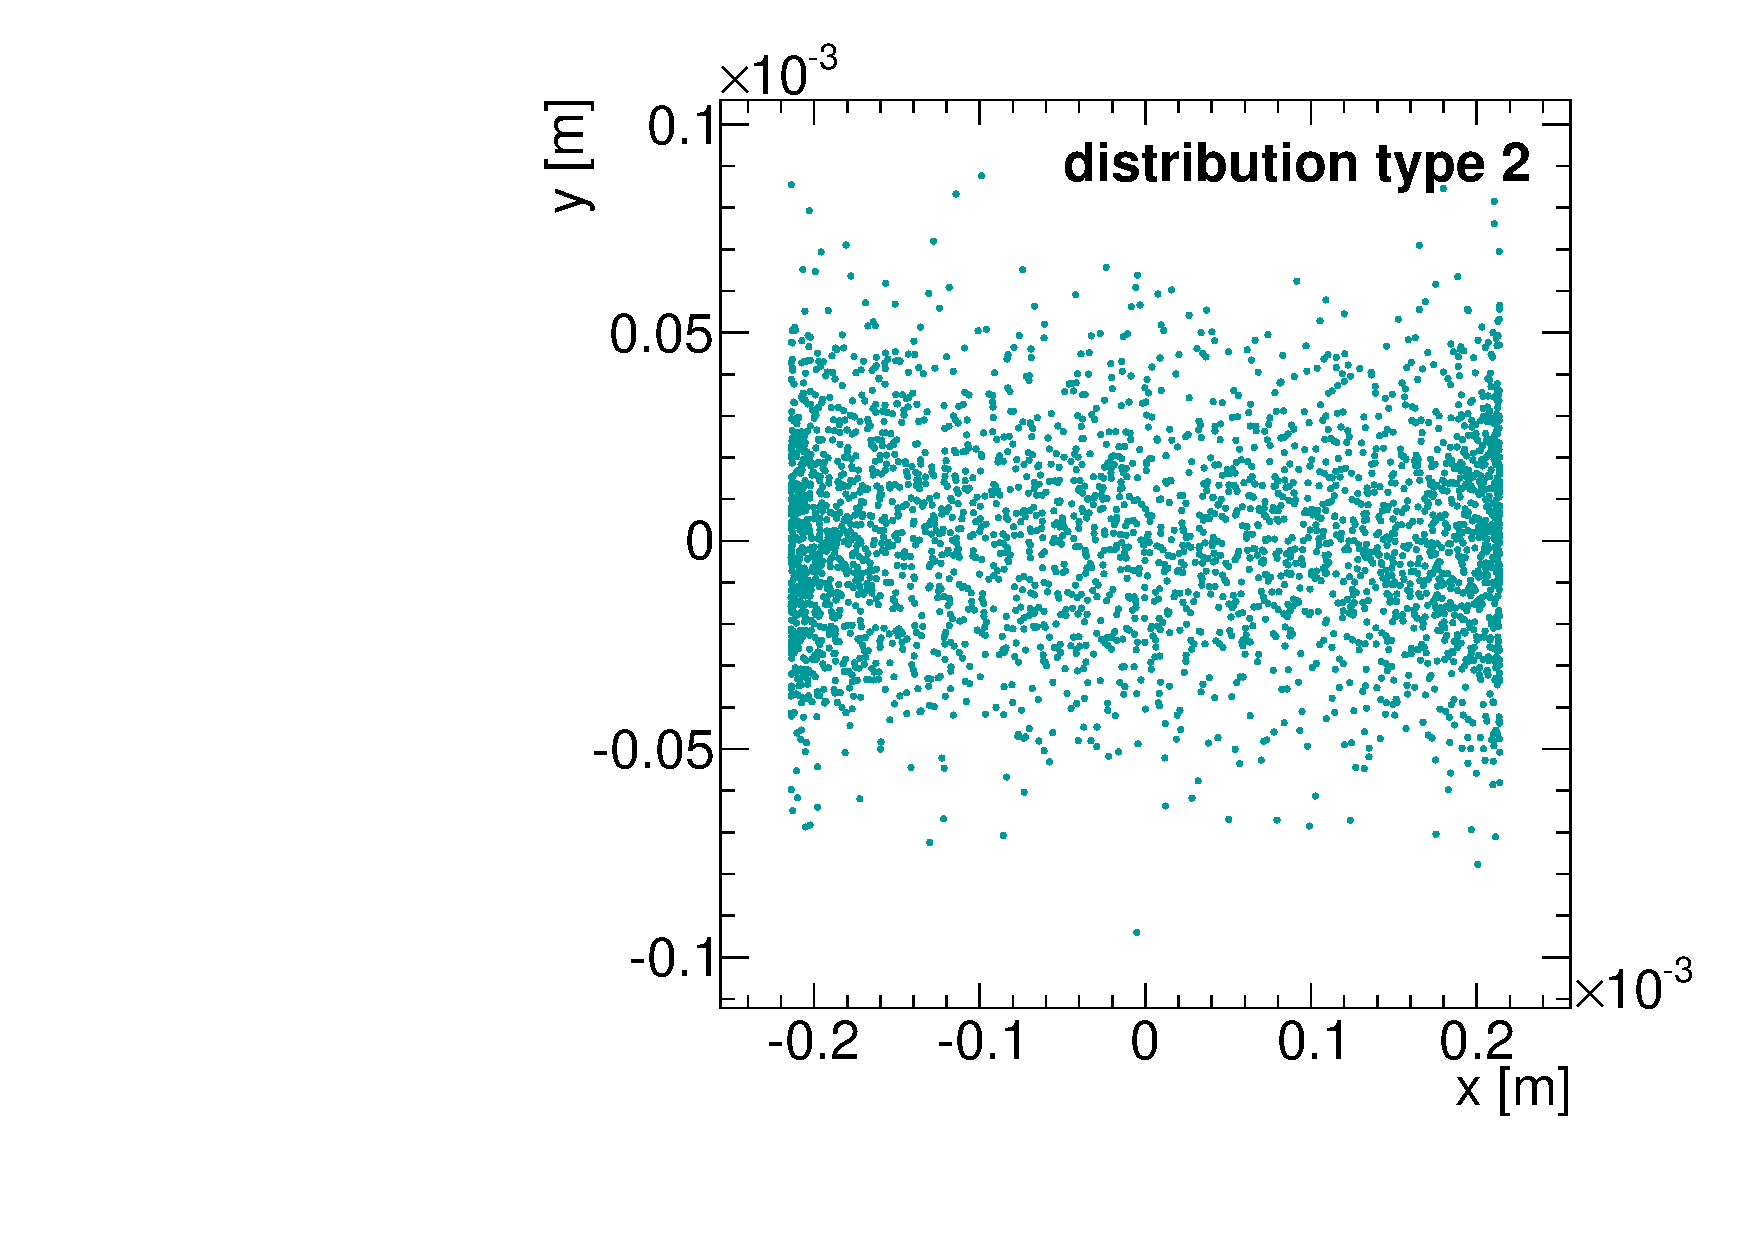
\includegraphics[width=0.48\textwidth]{figures/realspace_d2}
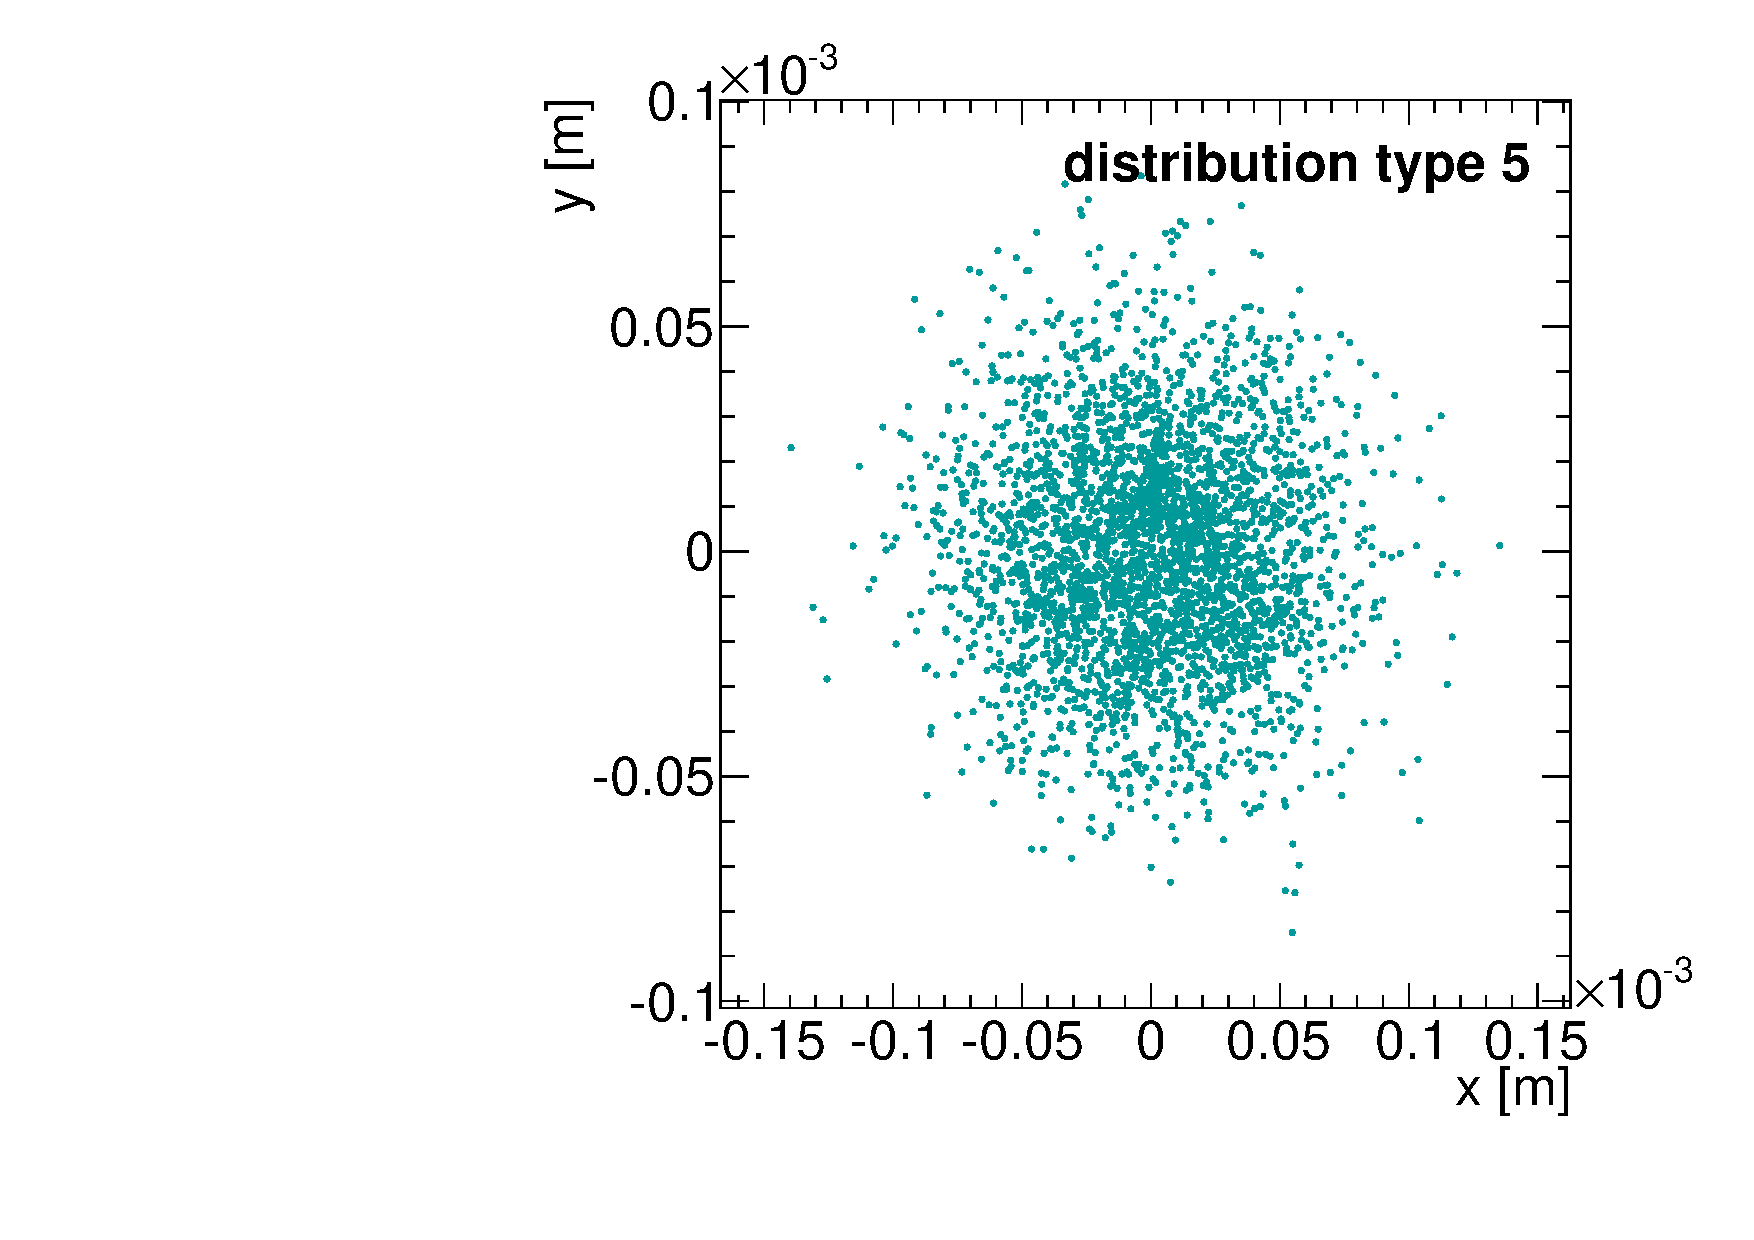
\includegraphics[width=0.48\textwidth]{figures/realspace_d5}
\end{center}
\begin{picture} (0.,0.)
\setlength{\unitlength}{1.0cm}
    \put (3.5,1){(a)}
    \put (10.5,1){(b)}
\end{picture}
\vspace{-1cm}
\caption{\textsf{Initial halo distribution of type 2 (a) and 5 (b). Data has been exracted from \texttt{dist0.dat}.}}
\end{figure}


\section{Post-processing}

\subsection{Create files with lost particles}

Three files are \textbf{input} to the program \texttt{BeamLossPattern}. The source files are {\href{http://lhc-collimation-project.web.cern.ch/lhc-collimation-project/BeamLossPattern.htm}{here}}.

\begin{enumerate}
\item The output file from the previous step \texttt{tracks2.dat}. 
\item A file that is originally produced by MadX. It contains essentially 

\begin{itemize}
\item aper\_1 = half width rectangle
\item aper\_2 = half height rectangle
\item aper\_3 = half horizontal axis ellipse (or radius if circle)
\item aper\_4 = half vertical axis ellipse
\end{itemize}

as a function of $s$. 

\item \texttt{SurveyWithCrossing\_XP\_lowb.dat} This file is not explicitly handed over as an argument, but needed nevertheless. It contains the offset between aperture centre and circulating beam as function of the longitudinal coordinate along the accelerator. Most of the time this is zero - exceptions are in the experimental IRs if there's a crossing angle active and in the separation/recombination dipoles.
\end{enumerate}

With two more arguments, \textit{lowb} for collimator settings in collision mode, and \textit{BLP\_out} to create the output, the command could look like \\

\texttt{./BeamLossPattern\_2005-04-30\_gcc2.9 lowb tracks2.dat BLP\_out allapert.b1}\newline

and \texttt{BeamLossPattern} creates two files:

\begin{enumerate}
\item \texttt{LP\_BLP\_out.s}
\item \texttt{LPI\_BLP\_out.s} The colums are \texttt{1=name, 2=turn, 3=s, 4=x, 5=xp, 6=y, 7=yp, 8=dE/E, 9=type, 10=turns in machine after first hits on collimators}
\end{enumerate}
The difference is merely in the resolution, the second one has a resolution of 0.1~m. Each line corresponds to one absorbed particle. The third colum indicates the position of the lost particle in meters. 
\subsubsection{Current Bug}
The current executable needs to be fixed and recompiled in order to avoid the output of binary character (due to incompatibility of the BeamLossPattern code and SL5 and the default installation on lxplus with SL6. A work-around would be the following command which should already included in the job scripts:\\
\texttt{perl -pi -e $'$s/\textbackslash0/ /g$'$ LPI\_BLP\_out.s}


\subsection{Clean Inelastics}

As aperture information was only available when the \texttt{BeamLossPattern} program was executed, several files need to be cleaned from particles that were actually absorbed in the collimators or lost elsewhere. This information is in the \texttt{LP*\_BLP\_out.s} files and is used as input to the next program, \texttt{CleanInelastic}.

The following are the \texttt{input} files:

\begin{enumerate}
\item \texttt{coll\_summary.dat} 

\item \texttt{LPI\_BLP\_out.s} Lost particle from BeamLossPattern.
\item \texttt{CollPositions.b1.dat} Initial input to be provided (?) with the collimator index, its name and position in meters.
\item \texttt{FLUKA\_impacts.dat} This file contains still particles which would actually be lost on collimators. The first file is used to produce a file with real impacts only.
\end{enumerate}

The \textbf{output} files are:

\begin{enumerate}

\item \texttt{impacts\_real.dat} Is a subset of \texttt{FLUKA\_impacts.dat} with only those particles in it which are actually lost on the collimators.
\item \texttt{impacts\_fake.dat} 
\end{enumerate}

\subsection{Correction of the collimation summary}

In the last step, \texttt{impacts\_fake.dat} is used to update the output \texttt{coll\_summary.dat} from lost particles. A dedicated script, \texttt{correct\_coll\_summary.sh} does it for you.
\end{document}  
